\documentclass{article}%\documentclass[a0,portrait]{a0poster}
\usepackage[a0paper,margin=5mm,paper height=1200mm,paper width=700mm]{geometry}

\usepackage{stringstrings}
\usepackage{tikz,pgf}
\usetikzlibrary{intersections,calc}

%% FONTS
\setlength{\baselineskip}{2ex}
\font\signNameFont="Interstate" at 27pt
\font\signDescFont="Interstate" at 14pt
\font\mainTitleFont="Interstate" at 72pt
\font\secTitleFont="Interstate" at 60pt
\font\bottomTitleFont="Interstate" at 75pt
\font\specialSignFont="Interstate" at 20pt

\newcommand{\signName}[1]{\uppercase{\signNameFont #1}}
\newcommand{\signDesc}[1]{\uppercase{\signDescFont #1}}
\newcommand{\mainTitle}[1]{\uppercase{\mainTitleFont #1}}
\newcommand{\secTitle}[1]{\uppercase{\secTitleFont #1}}
\newcommand{\bottomTitle}[1]{\uppercase{\bottomTitleFont #1}}
\newcommand{\specialSign}[1]{\uppercase{\specialSignFont #1}}

%% POSITIONING
\newcommand{\baselineStart}{-123.5mm}
\newcommand{\baselineSkip}{-89.2mm}
\newcounter{SignColumn}

\newcommand{\firstrow}{
	\path(0,\baselineStart) coordinate(Baseline);
%	\draw[red, ultra thick, dashed]
%		let \n0={290mm} in (Baseline)++(-\n0,0)--++(2 * \n0,0);
	\foreach \X in {1,...,10} {
		\path
			let \n0={59.5mm} in
			(\n0 * \X - \n0 * 5.5, 0) coordinate(Column\X);
%		\draw[red, ultra thick, dashed]
%			(Column\X) ++(0,-10mm) -- ++(0,-1000mm);
	}
}
\newcommand{\newrow}{
	\path(Baseline) ++(0,\baselineSkip)coordinate(Baseline);
%	\draw[red, ultra thick, dashed]
%		let \n0={290mm} in (Baseline)++(-\n0,0)--++(2 * \n0,0);
	\setcounter{SignColumn}{0}
}

\newcommand{\bg}[2]{} % debug

\newcommand{\hsign}[3]{%
	\caselower[q]{#2}
	\edef\texname{signs/\thestring.tex}
	%
	\draw
		#3 coordinate(SignHere)
		(SignHere)++(0,#1)node{\begin{tikzpicture}[
			scale=0.75,
			ultra thick,
			line cap=round,
			line join=round
		]
			\InputIfFileExists{\texname}{}{}
		\end{tikzpicture}}
		;
}
\newcommand{\xsign}[2][0mm]{%
	\stepcounter{SignColumn}
	\edef\columnName{Column\theSignColumn}
	\hsign{#1}{#2}{%
		(\columnName) coordinate(Column)
		(Column |- Baseline)}
}

\newcommand{\sign}[3][\defname]{%
	\def\defname{\signName{#2}}
	\xsign[40mm]{#2}
	%
	\draw
		(SignHere)node[
			anchor=south,
			text width=55mm,
			align=center
		]{\signName{#1}}

		(SignHere)++(0,-0mm)node[
			anchor=north,
			text width=55mm,
			align=center
		]{\signDesc{#3}}
		;
}




\begin{document}
\centering
\begin{tikzpicture}
	\draw(0,0)node[anchor=north]{
%		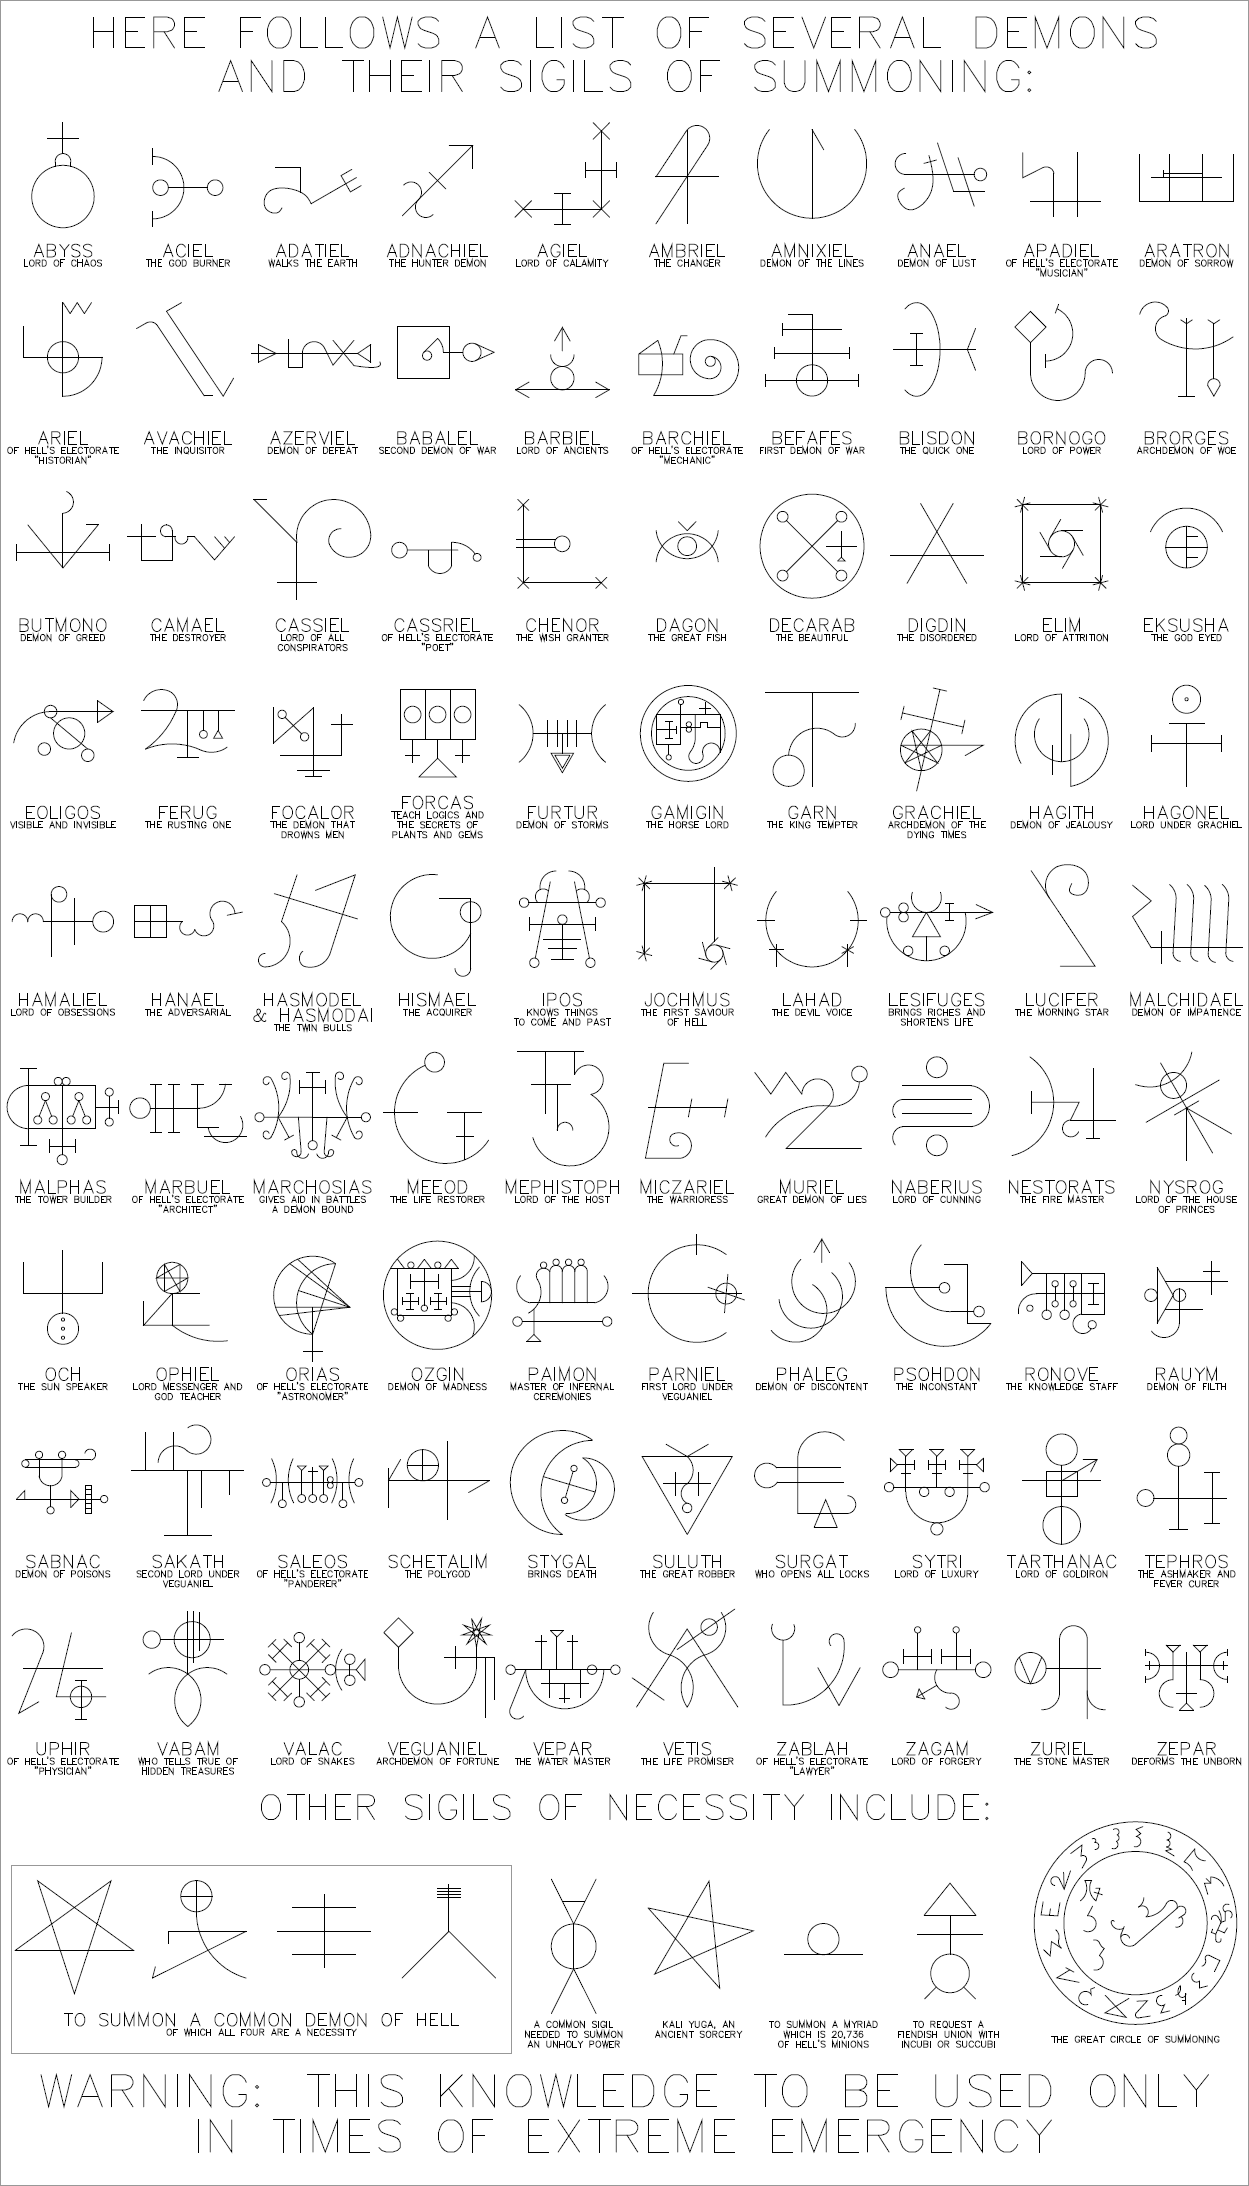
\includegraphics[scale=2.25]{summons-cropped.png}
	};

	\firstrow
	\sign{Abyss}{Lord of Chaos}
	\sign{Aciel}{The God Burner}
	\sign{Adatiel}{Walks the Earth}
	\sign{Adnachiel}{The Hunter Demon}
	\sign{Agiel}{Lord of Calamity}
	\sign{Ambriel}{The Changer}
	\sign{Amnixiel}{Demon of the Lines}
	\sign{Anael}{Demon of Lust}
	\sign{Apadiel}{of Hell's Electorate "Musician"}
	\sign{Aratron}{Demon of Sorrow}\newrow
	\sign{Ariel}{of Hell's Electorate "Historian"}
	\sign{Avachiel}{The Inquisitor}
	\sign{Azerviel}{Demon of Defeat}
	\sign{Babalel}{Second Demon of War}
	\sign{Barbiel}{Lord of Ancients}
	\sign{Barchiel}{of Hell's Electorate "Mechanic"}
	\sign{Befafes}{First Demon of War}
	\sign{Blisdon}{The Quick One}
	\sign{Bornogo}{Lord of Power}
	\sign{Brorges}{Archdemon of Woe}\newrow
	\sign{Butmono}{Demon of Greed}
	\sign{Camael}{The Destroyer}
	\sign{Cassiel}{Lord of all Conspirators}
	\sign{Cassriel}{of Hell's Electorate "Poet"}
	\sign{Chenor}{The Wish Granter}
	\sign{Dagon}{The Great Fish}
	\sign{Decarab}{The Beautiful}
	\sign{Digdin}{The Disordered}
	\sign{Elim}{Lord of Attrition}
	\sign{Ekusha}{The God Eyed}\newrow
	\sign{Eoligos}{Visible and Invisible}
	\sign{Ferug}{The Rusting One}
	\sign{Focalor}{The Demon that Drowns Men}
	\sign{Forcas}{Teach Logics and the Secrets of Plants and Gems}
	\sign{Furtur}{Demon of Storms}
	\sign{Gamigin}{The Horse Lord}
	\sign{Garn}{The King Tempter}
	\sign{Grachiel}{Archdemon of the Dying Times}
	\sign{Hagith}{Demon of Jealousy}
	\sign{Hagonel}{Lord under Grachiel}\newrow
	\sign{Hamaliel}{Lord of Obsessions}
	\sign{Hanael}{The Adversarial}
	\sign[Hasmodel \&~Hasmodai]{hasmodel}{The Twin Bulls}
	\sign{Hismael}{The Acquirer}
	\sign{Ipos}{Knows Things to Come and Past}
	\sign{Jochmus}{The First Saviour of Hell}
	\sign{Lahad}{The Devil Voice}
	\sign{Lesifuges}{Brings Riches and Shortens Life}
	\sign{Lucifer}{The Morning Star}
	\sign{Malchidael}{Demon of Impatience}\newrow
	\sign{Malphas}{The Tower Builder}
	\sign{Marbuel}{of Hell's Electorate "Architect"}
	\sign{Marchosias}{Gives Aid in Battles/A Demon Bound}
	\sign{Meeod}{The Life Restorer}
	\sign{Mephistoph}{Lord of the Host}
	\sign{Miczariel}{The Warrioress}
	\sign{Muriel}{Great Demon of Lies}
	\sign{Naberius}{Lord of Cunning}
	\sign{Nestorats}{The Fire Monster}
	\sign{Nysrog}{Lord of the House of Princes}\newrow
	\sign{Och}{The Sun Speaker}
	\sign{Ophiel}{Lord Messenger and God Teacher}
	\sign{Orias}{of Hell's Electorate "Astronomer"}
	\sign{Ozgin}{Demon of Madness}
	\sign{Paimon}{Master of Infernal Ceremonies}
	\sign{Parniel}{First Lord under Veguaniel}
	\sign{Phaleg}{Demon of Discontent}
	\sign{Psohdon}{The Inconstant}
	\sign{Ronove}{The Knowledge Staff}
	\sign{Rauym}{Demon of Filth}\newrow
	\sign{Sabnac}{Demon of Poisons}
	\sign{Sakath}{Second Lord under Veguaniel}
	\sign{Saleos}{of Hell's Electorate "Panderer"}
	\sign{Schetalim}{The Polygod}
	\sign{Stygal}{Brings Death}
	\sign{Suluth}{The Great Robber}
	\sign{Surgat}{Who Opens all Locks}
	\sign{Sytri}{Lord of Luxury}
	\sign{Tarthanac}{Lord of Goldiron}
	\sign{Tephros}{The Ashmaker and Fever Curer}\newrow
	\sign{Uphir}{of Hell's Electorate "Physician"}
	\sign{Vabam}{Who Tells True of Hidden Treasures}
	\sign{Valac}{Lord of Snakes}
	\sign{Veguaniel}{Archdemon of Fortune}
	\sign{Vepar}{The Water Master}
	\sign{Vetis}{The Life Promiser}
	\sign{Zablah}{of Hell's Electorate "Lawyer"}
	\sign{Zagam}{Lord of Forgery}
	\sign{Zuriel}{The Stone Master}
	\sign{Zepar}{Deforms the Unborn}

	\draw(0,-8mm)node[anchor=north,align=center]{%
		\mainTitle{Here follows a List of several Demons}\\%
		\mainTitle{and their Sigils of Summoning:}};

	\draw(Baseline)++(0,-18mm)node[anchor=north]{%
		\secTitle{Other Sigils of necissity include:}};
	\newrow
	\newcommand{\TextHere}{++(0,-30mm)}

	\xsign{common1}
	\xsign{common2}
	\xsign{common3}
	\xsign{common4}
	\draw ($(Column2)!0.5!(Column3)$) coordinate(Column25)
	(Column25 |- Baseline)\TextHere node[anchor=north]{%
		\specialSign{TODO}};

	\xsign{unholy}
	\draw (SignHere)\TextHere node[anchor=north, text width=55mm, align=center]{%
		\specialSign{A common Sigil needed to summon an Unholy Power}};

	\xsign{kaliyuga}
	\draw (SignHere)\TextHere node[anchor=north]{%
		\specialSign{An Ancient Sorcery}};

	\xsign{myriad}
	\draw (SignHere)\TextHere node[anchor=north, text width=55mm, align=center]{%
		\specialSign{To summon a Myriad which is 20,736 of Hell's Minions}};

	\xsign{union}
	\draw(SignHere)\TextHere node[anchor=north, text width=55mm, align=center]{%
		\specialSign{To request a fiendish Union with Incubi or Succubi}};

	\hsign{10mm}{circle}{%
		($(Column9)!0.5!(Column10)$) coordinate(Column95)
		(Column95 |- Baseline)}
	\draw(SignHere)\TextHere node[anchor=north]{%
		\specialSign{The Great Circle of Summoning}};

	\draw(Baseline)++(0,-80mm)node[align=center]{%
		\bottomTitle{Warning: This knowledge to be used only}\\%
		\bottomTitle{in times of extreme emergency}}
		
	;
\end{tikzpicture}
\end{document}
